%====================================================================================================
\chapter{Introduction} \label{ch:introduction}
%====================================================================================================
The Standard Model of elementary particle physics (\SM) is a remarkably successful theoretical framework, describing the known fundamental particles and their interactions via the electromagnetic, weak, and strong forces. It has been continuously validated through decades of experimental results and provides precise predictions that agree very well with observations.

However, the SM is not a complete theory of nature. It does not incorporate gravity, nor does it provide an explanation for the existence of dark matter or the origin of neutrino masses. These open questions motivate the search for new physics beyond the Standard Model.

To probe these fundamental questions, high-energy particle colliders are indispensable, as they enable us to access shorter distance scales and higher energy regimes where rare physics phenomena are more likely to manifest. The Large Hadron Collider (LHC), located at CERN, is a proton-proton collider with a center-of-mass energy of 14~TeV, designed to investigate fundamental interactions and to search for phenomena beyond the SM. The LHC hosts four major experiments—ATLAS, CMS, ALICE, and LHCb—each designed to investigate different aspects of high-energy physics.

After the discovery of the Higgs boson in 2012 at LHC, the LHC faces more challenges in probing high energy physics phenomena. To enable the exploration of new physics, including the measurement of the Higgs boson self-coupling or precise determination of the Higgs boson with vector boson and fermions, much larger statistical samples are required. Currently, the LHC is undergoing a comprehensive upgrade to the High-Luminosity LHC (\HL-LHC). This upgrade, called Phase-II upgrade, aims to increase the instantaneous luminosity by a factor of five to seven, allowing more collision events to be recorded and improving the precision of physics measurements.

The following sections in this chapter provide an overview of the LHC, the ATLAS experiment, and the upcoming Phase-II upgrade for the High-Luminosity LHC, followed by the motivation of the studies in this thesis.
%====================================================================================================
\section{The Large Hadron Collider} \label{sec:LHC}
%====================================================================================================
The Large Hadron Collider (LHC) is a hadron collider of the highest energy in the world, located about 100~m underground at the European Organization for Nuclear Research (CERN) near Geneva, Switzerland. It has a 27-kilometer circular tunnel, crossing the border between Switzerland and France. The LHC was designed to explore the frontiers of high-energy physics by colliding protons and occasionally heavy ions, such as lead nuclui.

Protons are first accelerated using a series of smaller accelerators—like the LINAC, Proton Synchrotron (\PS), and Super Proton Synchrotron (SPS)—before being injected into the LHC ring, where they are further accelerated. The LHC can achieve a center-of-mass energy of up to 14~TeV in proton-proton collisions currently, and is capable of delivering instantaneous luminosity of about $2 \times 10^{34}~\mathrm{cm}^{-2}\mathrm{s}^{-1}$. Figure~\ref{fig:LHC_complex} provides an overall view of the LHC complex.

\begin{figure}[htbp]
  \centering
  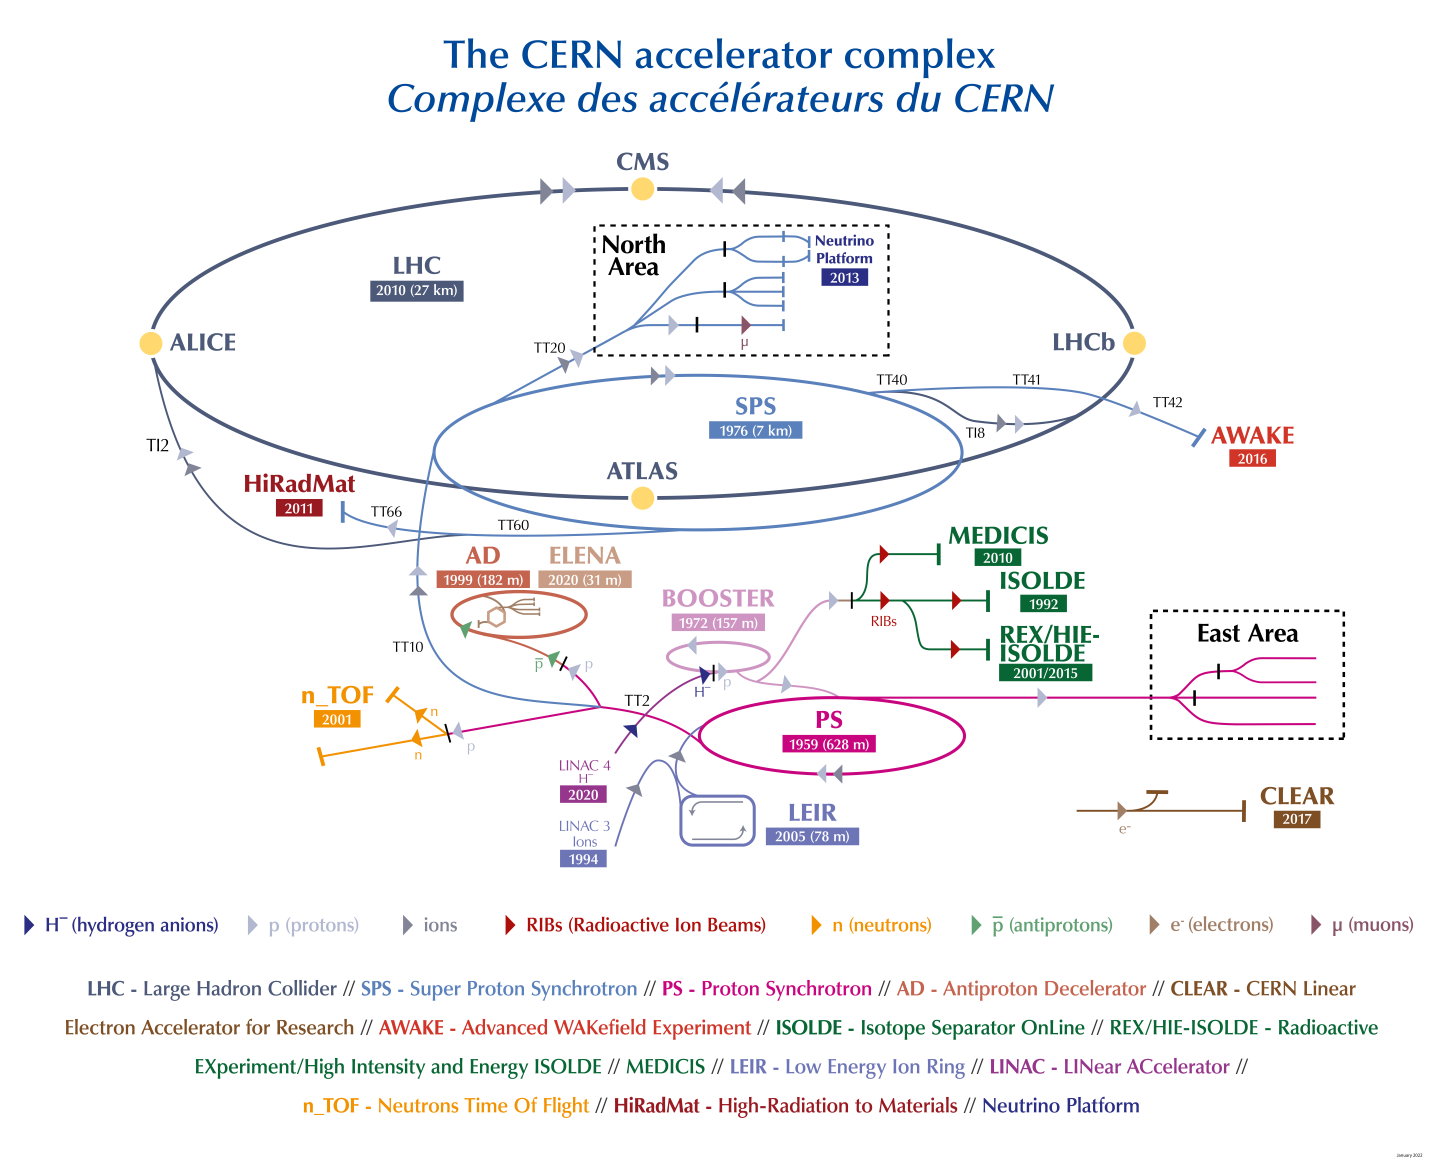
\includegraphics[width=1.0\textwidth]{figs/chapter1/LHC_complex.png}
  \caption{Overview of the LHC accelerator complex, illustrating the main accelerator ring and the injector chain responsible for preparing and accelerating the particles prior to collision. \cite{LHCComplex}.}
  \label{fig:LHC_complex}
\end{figure}

One of the most significant achievements of the LHC to date is the discovery of the Higgs boson in 2012 by the ATLAS and CMS collaborations. This long-sought particle completes the Standard Model by confirming the mechanism of electroweak symmetry breaking through the Higgs field, explaining the generation of particle masses.

In the following, a brief overview of the four LHC experiments mentioned above is provided: ATLAS and CMS, which are general-purpose detectors designed to study a wide range of phenomena including Higgs boson production, Supersymmetry, and other physics beyond the SM; ALICE, which specializes in the study of the quark-gluon plasma in heavy-ion collisions; and LHCb, which specializes in rare decays involving $b$-quarks, for purposes such as measurements of CP violation.
%====================================================================================================
\section{The LHC-ATLAS Experiment} \label{ATLAS}
%====================================================================================================
The ATLAS (A Toroidal LHC ApparatuS) experiment is a general-purpose particle detector experiment located at one of the four main interaction points of the LHC, designed to explore a wide range of physics phenomena. It is composed of several sub-detector systems arranged concentrically around the beam interaction point. Starting from the innermost region, the \textit{Inner Detector}, immersed in a solenoidal magnetic field, is designed to tracks charged particles and reconstructs their momenta, as well as determining the position of vertices of the hardest scattering, that is, the primary collision with the highest momentum transfer in the event. Surrounding the Inner Detector, the \textit{Calorimeter} system consists of electromagnetic and hadronic calorimeters, which measure the energy of electrons, photons, and hadrons through their interactions with dense absorber materials such as lead and steel. The outermost layer is the \textit{Muon Spectrometer}, which detects muons that penetrate the inner layers, measuring their curvature in toroidal magnetic fields to determine their momenta. The solenoidal magnetic field in the inner region, combined with the toroidal magnetic fields in the outer region, forms the \textit{Magnet System} and allows for precise momentum measurements over a wide energy range. A two-level trigger system is used to select events. In current LHC Run3 phase, the first-level trigger is implemented in hardware and uses a subset of the detector information to accept events at a rate below 100 kHz, which is followed by a software-based trigger that reduces the accepted event rate to 1 kHz. A cut-away view of the ATLAS detector is shown in Figure~\ref{fig:ATLASDetector}. A detailed description of the ATLAS detector will be provided in Chapter~\ref{ch:ATLAS}.
\begin{figure}[htbp]
  \centering
  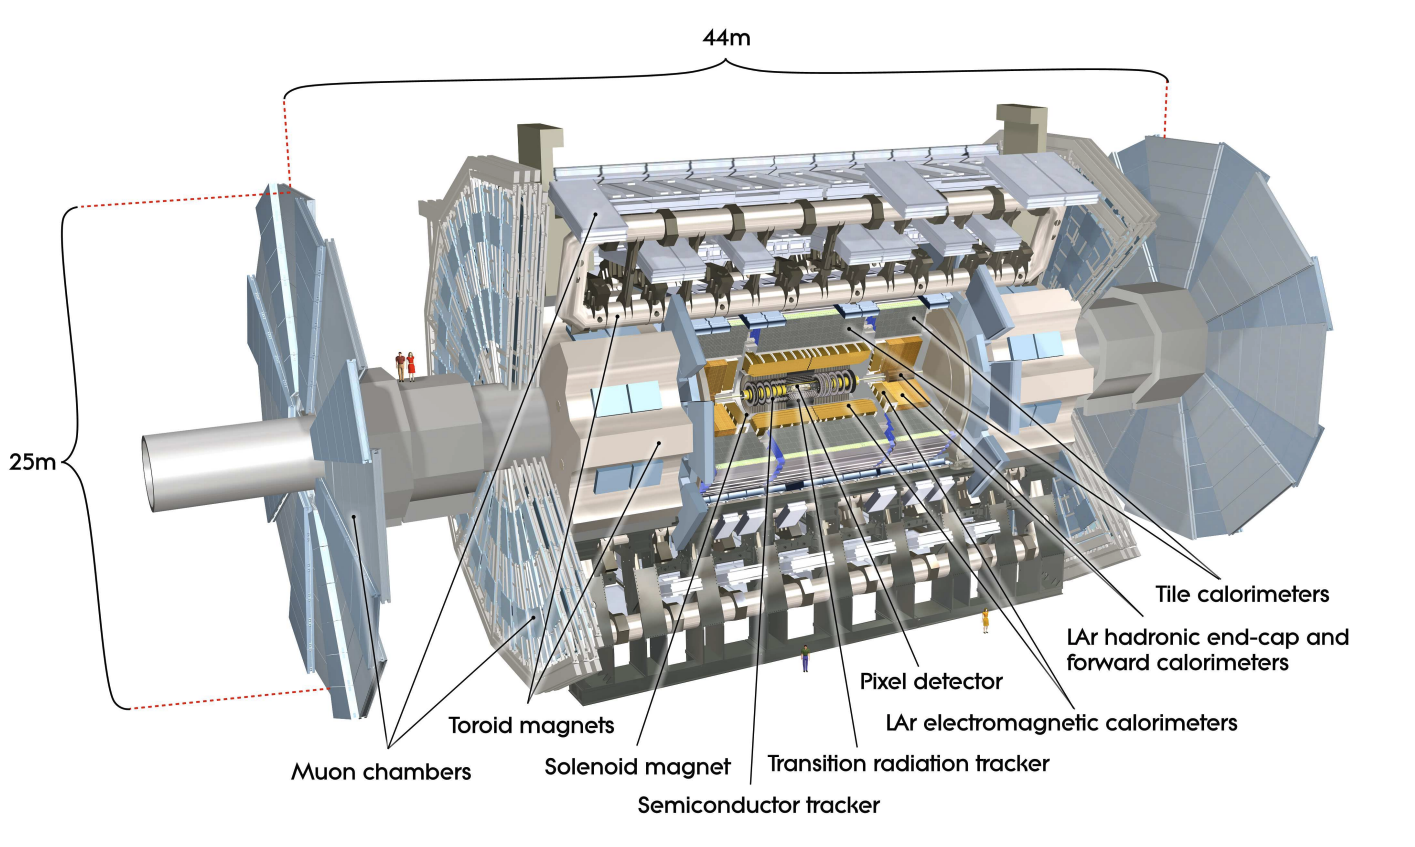
\includegraphics[width=1.0\textwidth]{figs/chapter1/ATLAS.png}
  \caption{Cut-away view of the ATLAS detector \cite{ATLASDetector2008}.}
  \label{fig:ATLASDetector}
\end{figure}
%====================================================================================================
\section{Phase-II Upgrade for HL-LHC} \label{sec:upgrade}
%====================================================================================================
To enhance the sensitivity to rare processes and potential signs of physics beyond the SM, the LHC has experienced a series of upgrades to increase event rate and improve the performance of detectors: Long Shutdown 1 (LS1) from 2013 to 2015, Long Shutdown 2 (LS2) from 2018 to 2022. Currently, an upcoming LS3---a comprehensive upgrade to for the LHC to the High-Luminosity LHC (HL-LHC)---is underway. This upgrade, also known as \textit{Phase-II upgrade}, scheduled to start around 2026 and finish at 2030, will lead the current Run~3 phase to the Run~4 phase of the LHC, as shown in Fig~\ref{fig:HL-LHC},

\begin{figure}[htbp]
  \centering
  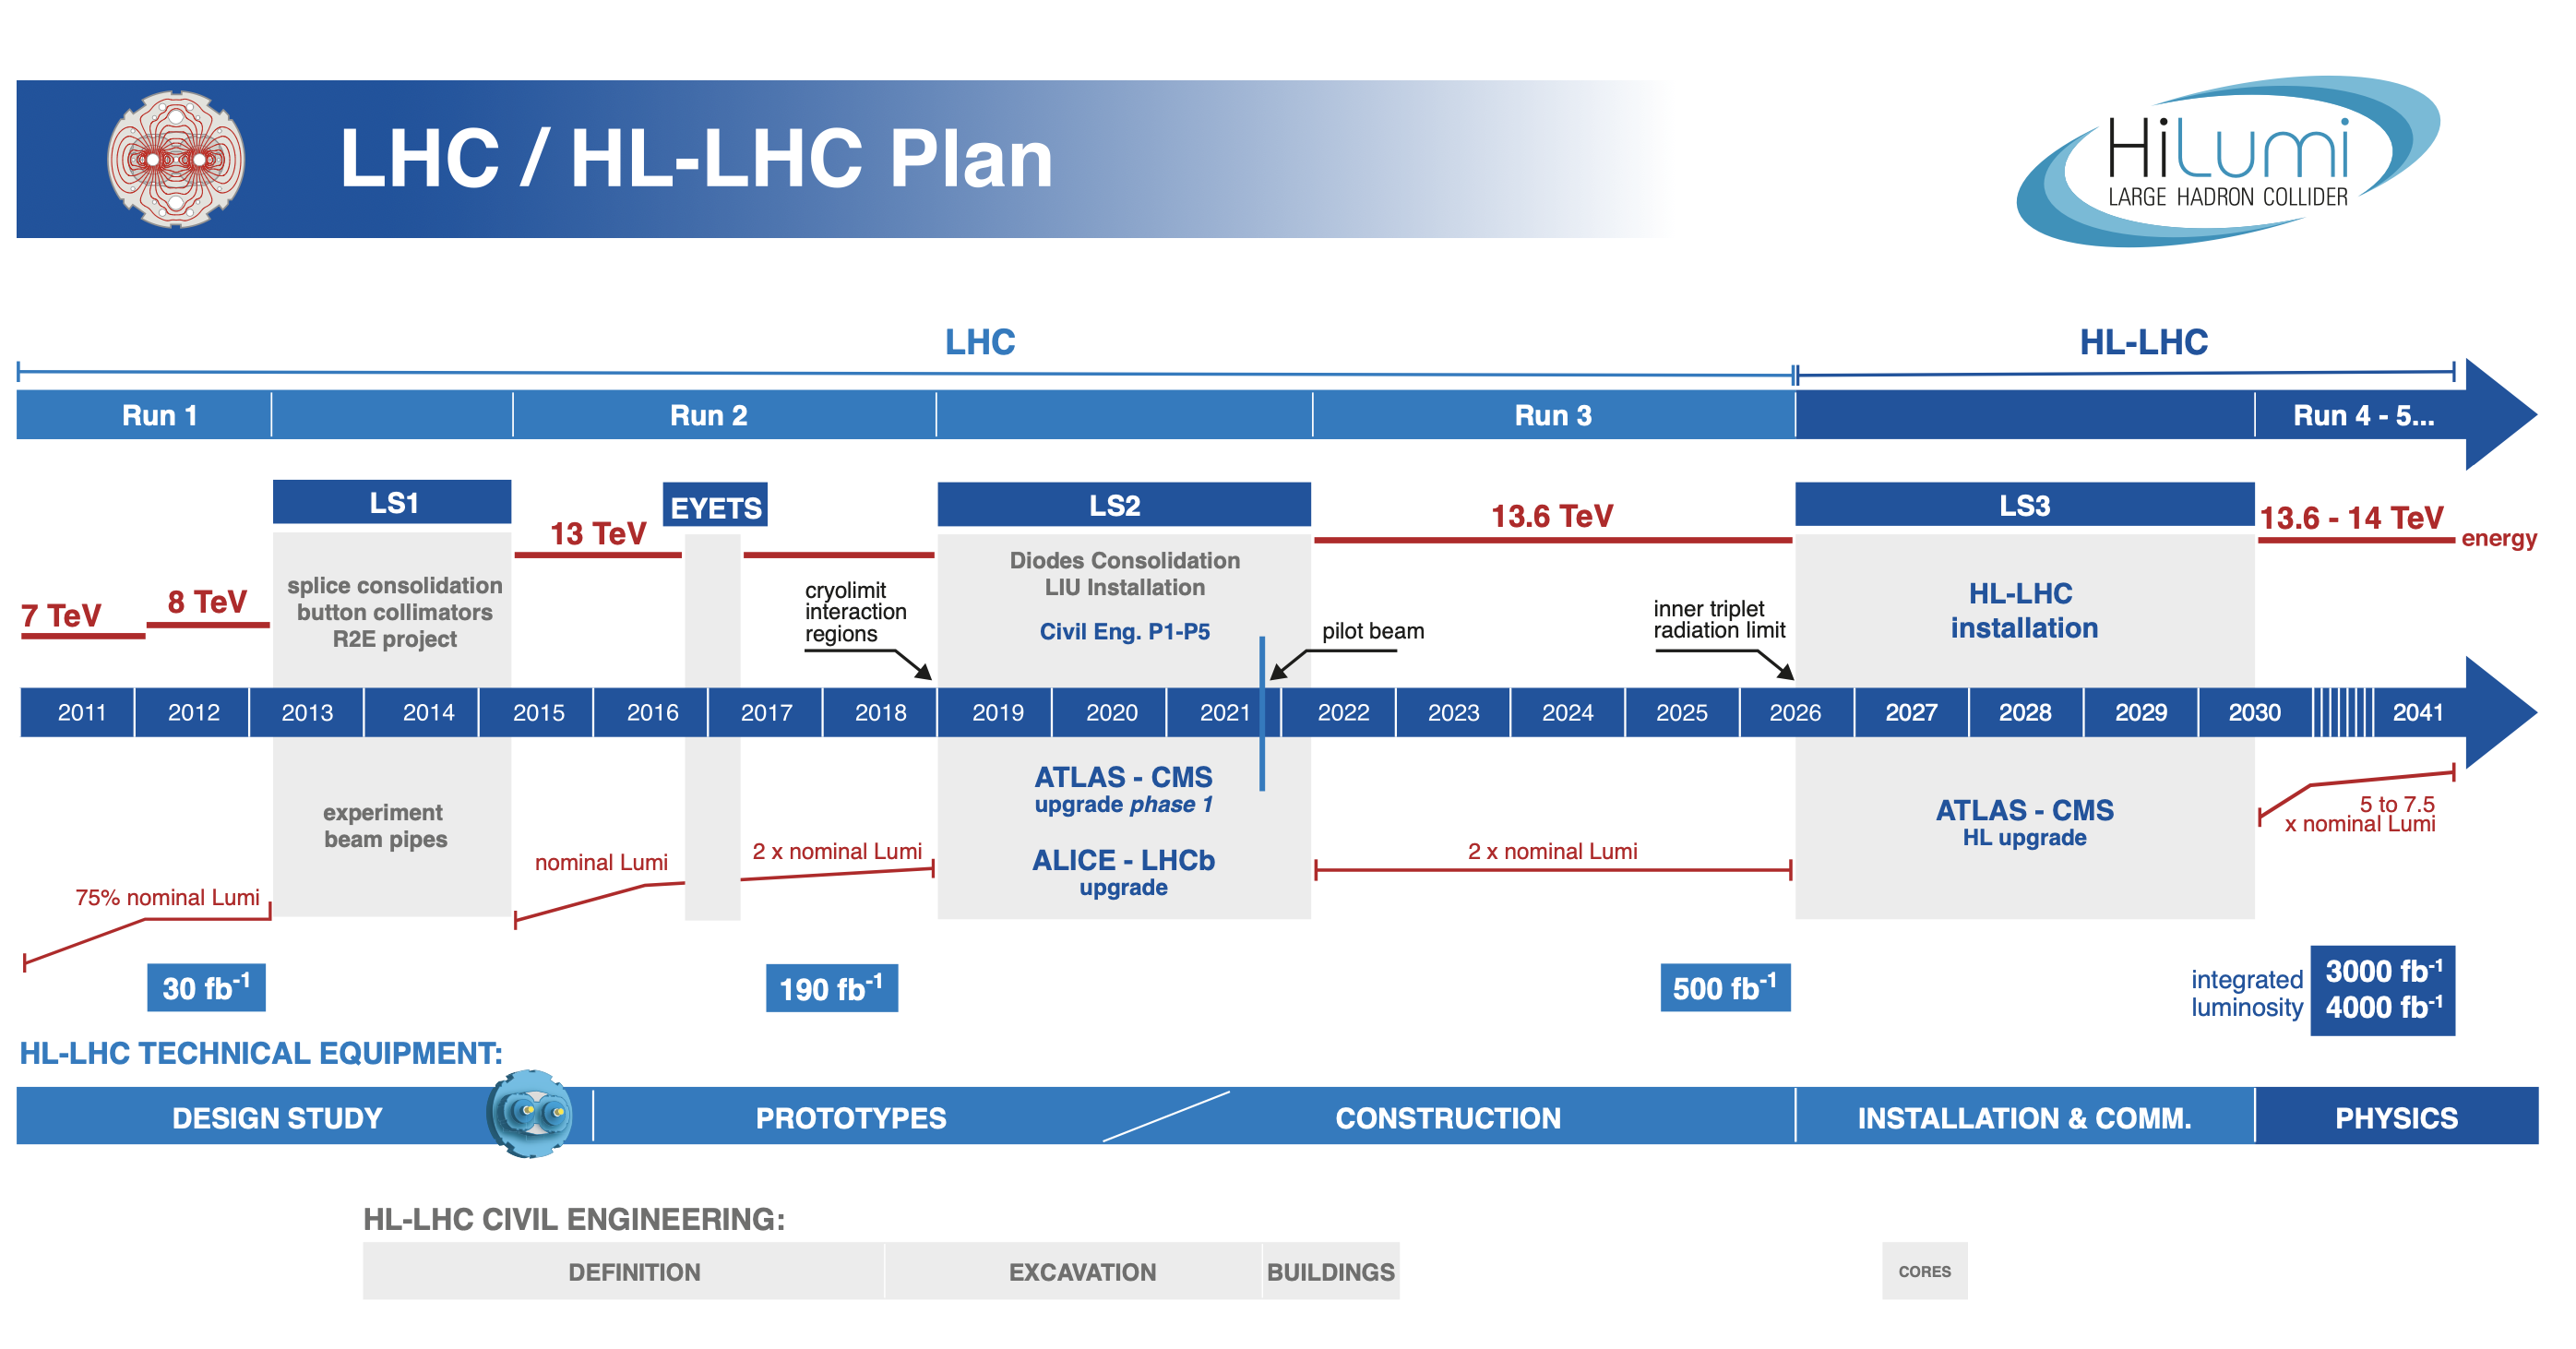
\includegraphics[width=1.0\textwidth]{figs/chapter1/HL-LHC_plan.pdf}
  \caption{HL-LHC schedule (last update January 2025) \cite{HL-LHC}.}
  \label{fig:HL-LHC}
\end{figure}

The instantaneous luminosity will be enhanced from the current $\sim 2 \times 10^{34}~\mathrm{cm}^{-2}\mathrm{s}^{-1}$ to a peak of $5$–$7.5 \times 10^{34}~\mathrm{cm}^{-2}\mathrm{s}^{-1}$ by increasing the number of protons per bunch and further focusing the beam at the collision points. Over a projected 10-year data-taking period, the HL-LHC is expected to deliver an integrated luminosity of up to $3000~\mathrm{fb}^{-1}$. This increase in luminosity will result in a much higher number of simultaneous proton-proton interactions per bunch crossing, known as \textit{pile-up}, rising from an average of 50–65 in Run~3 to 150–200 during HL-LHC operations (Run~4).

Such a large number of pile-ups poses a challenge to detectors in event reconstruction and background suppression processes. To meet these demands, the ATLAS detector will also undergo a upgrade to nearly all its major subsystems (sub-detectors). In the context of this research, particular attention is given to the relevant upgrades — including improvements to the muon system and the trigger and data acquisition (\TDAQ) system, which will be discussed in detail in Chapter~\ref{ch:ATLAS}.

%====================================================================================================
\section{Motivation and Structure of this Thesis} \label{sec:motivation}
%====================================================================================================
This thesis focuses on the development of the software simulation for the upgraded muon trigger system in the ATLAS experiment for the HL-LHC. To meet the requirements for the higher luminosity operation, the ATLAS muon trigger system will undergo a major upgrade. As a part of that, the Thin Gap Chamber (\TGC), at the endcap region of the muon system, will have its digital electronics and firmware logic entirely replaced and upgraded. As part of this upgrade, software simulation is necessary for validation and development and debugging of the firmware. In order to make the simulation feasible in the muon trigger chain, a corresponding software simulator needs to be implemented on ATLAS software framework, \textit{Athena}. Figure~\ref{fig:L0_trigger_chain} gives the Athena package scheme for whole simulation of the muon trigger chain. This thesis focuses on the development and the implementation for the \textit{Level-0 TGC Sector Logic} software package.

\begin{figure}[htbp]
  \centering
  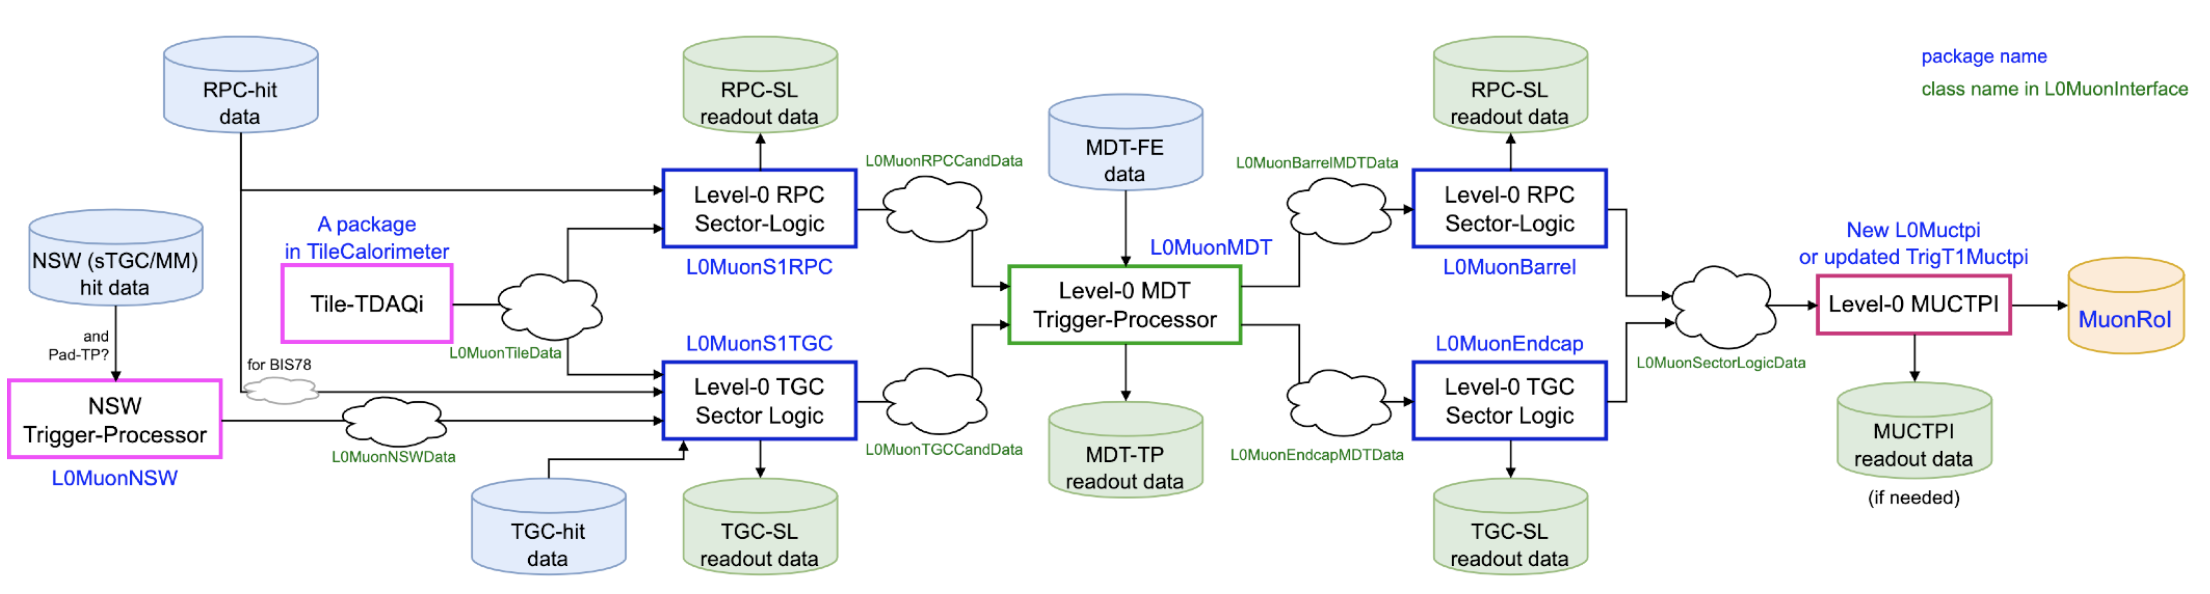
\includegraphics[width=1.0\textwidth]{figs/chapter1/L0_trigger_chain.png}
  \caption{A possible Athena package scheme for simulation of muon trigger chain for HL-LHC running (by J.Maeda).}
  \label{fig:L0_trigger_chain}
\end{figure}

The main challenge of the implementation is the significant memory usage. There is an existing \textit{bitwise simulator}, which emulates the firmware behavior of the TGC Sector Logic (SL) board, responsible for computing the muon transverse momentum based on the hit pattern combinations. While this approach can reporduce the SL calculation exactly, a single bitwise simulator consumes approximately 296~MB of memory, yet it covers only 1/48 of the TGC region. Consequently, extrapolating this to the full endcap region would result in a total memory usage of
\[
48 \times 296~\text{MB} \simeq 14~\text{GB},
\]
which is much higher than the current acceptable memory limit of about 500~MB for endcap muon trigger simulation on Athena.

Thereby, to support downstream developments such as the \textit{Level-0 MDT Trigger-Processor} package in the Figure~\ref{fig:L0_trigger_chain} following the \textit{Level-0 TGC Sector Logic}, we developed a simple emulator with minimal memory usage as a preliminary step of this research. This emulator generates trigger information for the next stage of the simulation using a Gaussian-based smearing algorithm. Subsequently, a simple simulation for trigger acceptance was implemented to bring the emulator closer to reality. However, the emulator still lacks the ability to reproduce actual physical phenomena, since the actual SL momentum calculation exhibits non-Gaussian characteristics. It confirms, as a result, the necessity for a high-precision simulator that can reproduce the trigger behavior for the L0 TGC Sector Logic on Athena.

Therefore, as the core of this research, the development of simulation of the endcap TGC Sector Logic (\SL), which is assigned to ATLAS Japan group, was performed on the base of the bitwise simulator. In this part, a bitwise-level simulator was locally extended and implemented into the Athena framework, simulating consistent logic behavior with the actual SL. A first attempt for optimizing the storage of Look-Up Table (LUT) was also applied to address the memory limitation. The result of the simulation is compared to stand-alone bitwise simulator.

This thesis is structured as follows: Chapter~\ref{ch:ATLAS} provides an overview of the LHC-ATLAS experiment, along with the upgrade for the HL-LHC. Chapter~\ref{ch:Athena} briefly introduces the ATLAS software framework, Athena. Chapter~\ref{ch:L0MuonEmulator} presents the development and the update to the simple emulator for L0 muon trigger system, followed by an assessment of its performance. Chapter~\ref{ch:L0MuonS1TGC} describes the implementation and optimization of the simulator for the TGC Sector Logic. Chapter~\ref{ch:conclusion} presents the conclusions of this research and discusses future prospects for further development and applications.